\chapter{Topin}

Durante o processo de desenvolvimento de um projeto, inúmeras ferramentas são utilizadas para auxiliar os membros da equipe de desenvolvimento a minimizar os possíveis problemas que a aplicação venha a possuir. Este capítulo tem o intuito de descrever as tecnologias utilizadas para a construção do projeto, bem como demonstrar as características da solução desenvolvida.

\section{Análise de Requisitos}

\subsection{Requisitos Funcionais}

Nesta seção serão descritas as principais funcionalidades referentes ao sistema de informação Topin, contudo os requisitos serão separados de forma a melhorar o entendimento sobre a aplicação como um todo, dividindo os requisitos referentes ao ambiente de gerenciamento das informações por parte da empresa prestadora de serviço de transporte público e a aplicação móvel disponibilizada para os passageiros.

\subsubsection*{Empresa de Transporte Público}

{\renewcommand{\arraystretch}{2}
\begin{table}[H]
\centering
\caption{Requisitos Funcionais do Administrador da Empresa de Transporte Público}
\label{tab:empresa-requisitos-funcionais}
\begin{tabular}{ l | p{13.5cm} }
\hline
\textbf{ID} & \textbf{História de Usuário} \\
\hline
RF001 & Como administrador da empresa preciso registrar as linhas disponíveis, atribuindo as coordenadas geográficas que determinam o caminho percorrido de cada linha.\\ \hline
RF002 & Como administrador da empresa preciso registrar as paradas de ônibus referenciadas pela sua geolocalização. \\ \hline
RF003 & Como administrador da empresa preciso registrar os horários de partidas de cada linha e o dia da semana que aquele horário está disponível. \\ \hline
RF004 & Como administrador da empresa preciso registrar marcadores de interesse ao uso de transporte público como pontos de venda de bilhetes. \\ \hline
RF005 & Como administrador da empresa preciso visualizar reclamações e sugestões advindas dos passageiros que enviaram por meio do aplicativo. \\ \hline
\end{tabular}
\legend{Fonte: Autor}
\end{table}

Na Tabela \ref{tab:empresa-requisitos-funcionais} são descritas em formato de histórias de usuário as funcionalidades essenciais para o gerenciamento do serviço de transporte público por parte da prestadora de serviço, entretanto apenas os requisitos que são importantes para o desenvolvimento da solução proposta nesse trabalho estão sendo listados.

\subsubsection*{Passageiro}

A seguir é possível observar a Tabela \ref{tab:passageiro-requisitos-funcionais} onde são colocados em evidência os principais requisitos para o funcionamento do aplicativo móvel para o passageiro, com o intuito de abordar os problemas que foram encontrados na pesquisa que pode ser melhor observada no Capítulo \ref{cap:metodologia}.

{\renewcommand{\arraystretch}{2}
\begin{table}[H]
\centering
\caption{Requisitos Funcionais do Passageiro}
\label{tab:passageiro-requisitos-funcionais}
\begin{tabular}{ l | p{13.5cm} }
\hline
\textbf{ID} & \textbf{História de Usuário} \\
\hline
RF001 & Como passageiro preciso consultar as linhas disponíveis para a cidade de Picos.\\ \hline
RF002 & Como passageiro preciso visualizar os horários e dias disponíveis para cada linha. \\ \hline
RF003 & Como passageiro preciso visualizar em um mapa o percurso e os pontos de parada para uma determinada linha. \\ \hline
RF004 & Como passageiro preciso visualizar as paradas mais próximas para entrar em um ônibus que esteja na linha desejada. \\ \hline
RF005 & Como passageiro preciso visualizar a minha posição atual no mapa para melhor me localizar em relação as paradas. \\ \hline
RF006 & Como passageiro preciso efetuar uma reclamação para as autoridades competentes por meio do aplicativo. \\ \hline
RF007 & Como passageiro preciso registrar minhas linhas favoritas, para facilitar o meu acesso evitando visualizar informações que não são de meu interesse. \\ \hline
RF008 & Como passageiro preciso visualizar as linhas disponíveis e os horários até quando não houver acesso a \textit{internet} disponível. \\ \hline
\end{tabular}
\legend{Fonte: Autor}
\end{table}

\subsection{Requisitos Não Funcionais}

Nesta seção serão descritos os principais requisitos não funcionais para obter uma melhor satisfação dos usuários em relação a utilização de transporte público, bem como restringir algumas tecnologias e comportamentos específicos para o desenvolvimento da aplicação, objetivando os recursos que cada tecnologia oferece em prol deste trabalho. Todavia os requisitos serão exibidos de forma categorizada com o intuito de melhorar o entendimento sobre os requisitos em cada ambiente, separando assim os requisitos em os que possuem relação com a aplicação dos administradores da empresa prestadora de serviço de transporte público e os referentes ao sistema de uso por parte dos seus passageiros.

\subsubsection*{Empresa de Transporte Público}

Na Tabela \ref{tab:empresa-requisitos-nao-funcionais} são descritas em formato de histórias de usuário as funcionalidades essenciais para o gerenciamento do serviço de transporte público por parte da prestadora de serviço, entretanto apenas os requisitos que são importantes para o desenvolvimento da solução proposta nesse trabalho estão sendo listados.

{\renewcommand{\arraystretch}{2}
\begin{table}[H]
\centering
\caption{Requisitos Não Funcionais do Administrador da Empresa de Transporte Público}
\label{tab:empresa-requisitos-nao-funcionais}
\begin{tabular}{ l | p{13.5cm} }
\hline
\textbf{ID} & \textbf{Descrição} \\
\hline
RNF001 & O sistema deve solicitar autenticação de usuário e senha para obter acesso. \\ \hline
RNF002 & O sistema deve funcionar para o ambiente \textit{web} de modo as ser compatível com os principais navegadores, como: Chrome, Firefox, Safari e \textit{internet} Explorer. \\ \hline
RNF003 & O sistema deve estar disponível 24 horas por dia e 7 dias por semana. \\ \hline
RNF004 & O sistema deve utilizar o sistema gerenciador de banco de dados PostgreSQL com a extensão PostGIS. \\ \hline
RNF005 & O sistema deve utilizar a linguagem de programação Python em conjunto com o \textit{framework} Django e sua biblioteca GeoDjango. \\ \hline
\end{tabular}
\legend{Fonte: Autor}
\end{table}

\subsubsection*{Passageiro}

Na Tabela \ref{tab:passageiro-requisitos-nao-funcionais} são descritas em formato de histórias de usuário as funcionalidades essenciais para o gerenciamento do serviço de transporte público por parte da prestadora de serviço, entretanto apenas os requisitos que são importantes para o desenvolvimento da solução proposta nesse trabalho estão sendo listados.

{\renewcommand{\arraystretch}{2}
\begin{table}[H]
\centering
\caption{Requisitos Não Funcionais do Passageiro}
\label{tab:passageiro-requisitos-nao-funcionais}
\begin{tabular}{ l | p{13.5cm} }
\hline
\textbf{ID} & \textbf{Descrição} \\
\hline
RNF001 & O aplicativo do passageiro deve funcionar para a plataforma Android, compatível com as versões acima da 4.4 KitKat. \\ \hline
RNF002 & O sistema deve possuir uma API para consultas de informações, utilizando a arquitetura REST e o formato de dados JSON. \\ \hline
RNF003 & O aplicativo deve armazenar os dados consultados à API utilizando o banco de dados pra disponibilizar os dados quando não houver conexão com a \textit{internet}. \\ \hline
RNF004 & A API deve estar disponível 24 horas por dia e 7 dias por semana. \\ \hline
RNF005 & A API deve suportar uma carga de acesso acima de 100 acessos simultâneos e mais de 10 mil consultas diárias. \\ \hline
RNF006 & O aplicativo deve funcionar de forma nativa a plataforma Android utilizando a linguagem de programação Java. \\ \hline
RNF007 & O aplicativo deve seguir as diretivas de interface do usuário descritas no Material Design\footnotemark. \\ \hline
\end{tabular}
\legend{Fonte: Autor}
\end{table}

\footnotetext{https://material.io/guidelines/}

\subsection{Modelagem do Sistema}

Ao término do levantamento de requisitos de qualquer \textit{software}, é impreterível a modelagem do sistema em virtude da dificuldade de entendimento das funcionalidades levantadas e, ao efetuar a modelagem do sistema facilita a compreensão do sistema por parte da equipe, bem como do próprio cliente, uma vez que comumente essa modelagem é feita por meio de diagramas UML que possibilitam uma visão gráfica do sistema, e não apenas textual.

Neste capítulo será possível visualizar dois dos principais diagramas da UML, o diagrama de classes e o diagrama de casos de uso. Tendo em vista a melhoria do entendimento reduziu-se os diagramas para demonstrar apenas o essencial para a compreensão da solução proposta por esse trabalho.

\subsubsection{Diagrama de Casos de Uso}

\subsubsection*{Empresa de Transporte Público}

Na análise efetuada no diagrama de casos de uso da Figura \ref{fig:caso-de-uso-administrador} é possível visualizar que o administrador da empresa é o responsável por garantir o pleno funcionamento da aplicação, pois ele teria a responsabilidade de gerenciar os dados mais importantes do sistema, contudo ainda se deve colocar em destaque três desses casos de uso:

\begin{lista}
\item \textbf{Gerenciar Linhas:} Consiste na manutenção das linhas atuais em que a empresa presta seus serviços. O administrador tem o dever de registrar as coordenadas geográficas referentes ao percurso do ônibus, bem como os seus horários de funcionamento em cada dia da semana.
\item \textbf{Gerenciar Marcadores:} Possibilita cadastrar pontos importantes para a melhor prestação do serviço, pois é a funcionalidade que permite que os administradores cadastrem as paradas de ônibus e os locais de venda de bilhetes para o uso do transporte público, bem como a localização desses pontos no mapa.
\item \textbf{Gerenciar Reclamações:} Permite que os administradores visualizem as reclamações efetuadas pelos passageiros por meio do aplicativo, assim, tendo a possibilidade de analisar de forma efetiva os problemas que ocorrem advindos do uso de transporte público.
\end{lista}

\begin{figure}[H]
\caption{Diagrama de Casos de Uso do Administrador}
\centering
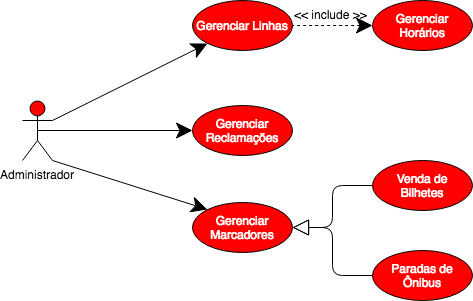
\includegraphics[width=0.7\textwidth]{imagens/caso-de-uso-administrador.png}
\legend{Fonte: Autor}
\label{fig:caso-de-uso-administrador}
\end{figure}

\subsubsection*{Passageiro}

O problema em torno deste trabalho visa a melhoria da experiência do passageiro para com o uso do transporte público. Após todo o estudo focado no problema em questão foi possível desenvolver o diagrama de casos de uso presente na Figura \ref{fig:caso-de-uso-passageiro}, que demonstra as funcionalidades básicas disponíveis para os passageiros baseadas nos seguintes casos de uso:

\begin{lista}
\item \textbf{Visualizar Linhas:} Possibilita ao passageiro visualizar uma lista de todas os percursos disponíveis para a cidade, bem como facilita o acesso a todos os horários disponíveis de cada percurso e, também, é permitido ao passageiro visualizar todo o percurso em um mapa.
\item \textbf{Visualizar Marcadores:} Consiste na disponibilização de uma interface onde é possível observar uma lista com todos os pontos importantes para o uso de transporte público, como por exemplo: paradas de ônibus e pontos de vendas de bilhetes. Além disso, também é possível visualizar a posição desses marcadores em um mapa.
\item \textbf{Efetuar Reclamação:} Permite aos passageiros de transporte público contatarem diretamente as pessoas responsáveis pelo transporte público, por meio de um formulário os usuários iram efetuar reclamações sobre a prestação do serviço de transporte público da cidade.
\end{lista}

\begin{figure}[H]
\caption{Diagrama de Casos de Uso do Passageiro}
\centering
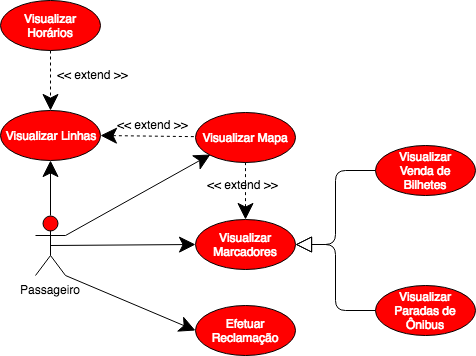
\includegraphics[width=0.7\textwidth]{imagens/caso-de-uso-passageiro.png}
\legend{Fonte: Autor}
\label{fig:caso-de-uso-passageiro}
\end{figure}

\subsubsection{Modelo Entidade-Relacionamento}

Como pode ser visto na Figura \ref{fig:modelo-entidade-e-relacionamento} o modelo de banco de dados foi criado de forma genérica para atender mais de uma empresa. A empresa será representada por meio da entidade do administrador, em que possibilita que todas as demais entidades estão relacionadas direta ou indiretamente com a empresa, assim, tornando possível que cada empresa gerencie apenas os dados referentes a ela. Este modelo também reduz algumas entidades e atributos adicionais que são utilizadas para o melhor funcionamento da solução, contudo não se fazem necessários para o entendimento do que será desenvolvido.

\begin{figure}[H]
\caption{Diagrama Entidade-Relacionamento}
\centering
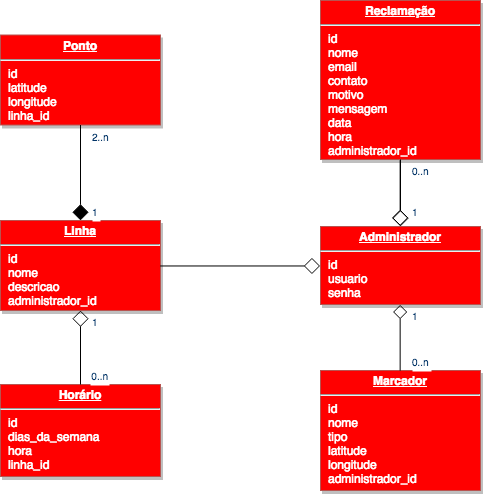
\includegraphics[width=0.7\textwidth]{imagens/modelo-entidade-e-relacionamento.png}
\legend{Fonte: Autor}
\label{fig:modelo-entidade-e-relacionamento}
\end{figure}

\section{Arquitetura do Software}

\subsection{Aplicativo Web}

Para o desenvolvimento da versão \textit{web} do aplicativo Topin, composta por um ambiente administrativo que possibilita o registro das informações necessárias para o funcionamento do sistema, foi utilizada a arquitetura de \textit{software} MTV que como pode ser visto na Figura \ref{fig:model-template-view} é dividida em três camadas:

\begin{figure}[H]
\caption{Arquitetura Model-Template-View}
\centering
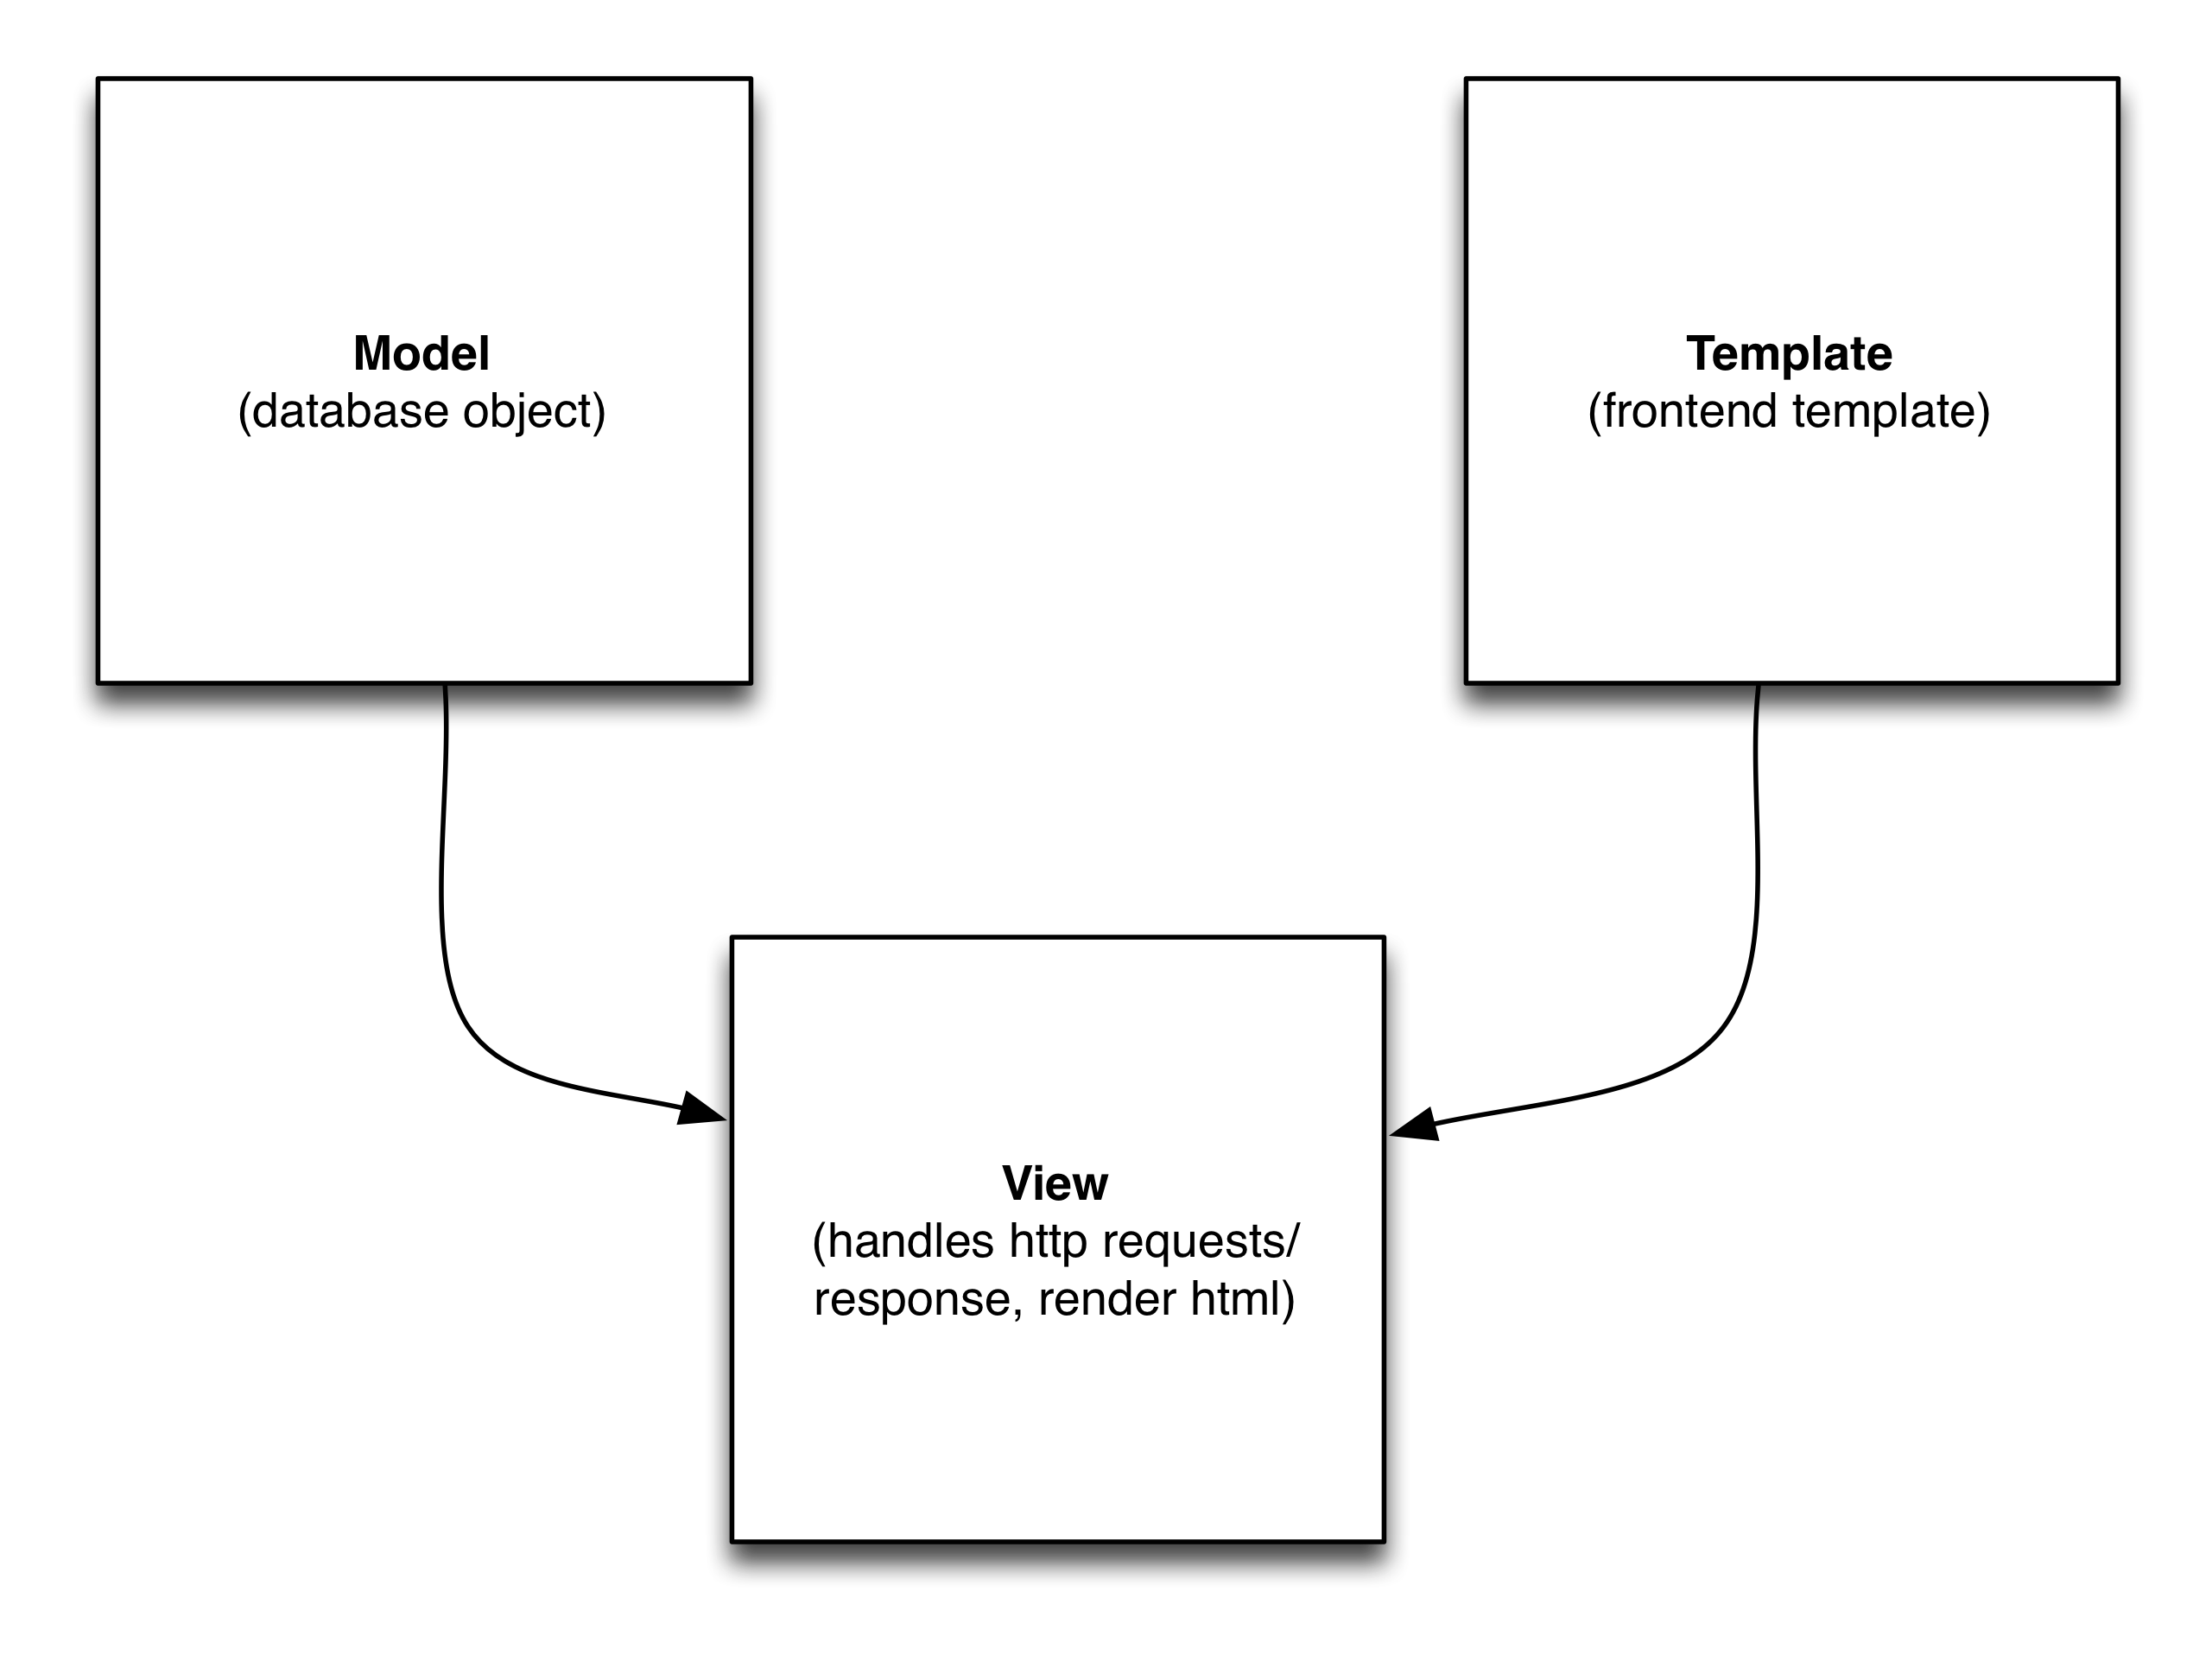
\includegraphics[width=.7\textwidth]{imagens/model-template-view.png}
\legend{Fonte: Cornell University}
\label{fig:model-template-view}
\end{figure}

\begin{lista}
\item \textbf{Model} é a única e definitiva fonte de acesso aos dados armazenados no banco de dados. Ele possui todos os campos e comportamentos essenciais dos dados que você está gerenciando no banco de dados.
\item \textbf{Template} é o meio de apresentação dos dados requisitados pelo usuário, geralmente esses dados são apresentados em uma página HTML ou em uma formatação de dados como JSON ou XML.
\item \textbf{View} é responsável pelas regras de negócio do sistema, bem como efetua o tratamento dos dados antes de serem enviados ao \textit{template}, ou seja, quando um usuário solicita algum serviço por meio de uma URL, a \textit{view} é quem deve efetuar os passos necessários para que o serviço seja executado.
\end{lista}

\subsection{Aplicativo Móvel}

O aplicativo para dispositivos móveis que visa atender as necessidades dos usuários de transporte público foi desenvolvido para a plataforma Android utilizando o padrão de arquitetura de \textit{software} MVP que como pode ser visto na Figura \ref{fig:model-view-presenter} é composto de três camadas:

\begin{lista}
\item \textbf{Model} é a representação abstrata das informações que serão armazenadas, sendo esta a camada que demonstra os campos que serão atualizadas pelo presenter quando houver modificações na view.
\item \textbf{View} é a camada visível ao usuário final do sistema, não contendo nenhuma regra de negócio, estando responsável apenas pela exibição e coleta de dados pelo usuário, disparando quando necessário a mudança de estado de informações ou eventos para o presenter, para que então o presenter altere o estado das informações, quando necessário, no banco de dados por meio do model ou então execute alguma ação com base na chamada de um evento.
\item \textbf{Presenter} é o intermédio entre o model e a view, estando encarregado de atualizar a view quando o model for alterado e sincronizar o model em relação a view. Como também possui a responsabilidade de efetuar o tratamento das informações antes de submeter a qualquer uma das camadas, sendo esta a camada onde é empregada as regras de negócio.
\end{lista}

\begin{figure}[H]
\caption{Arquitetura Model-View-Presenter}
\centering
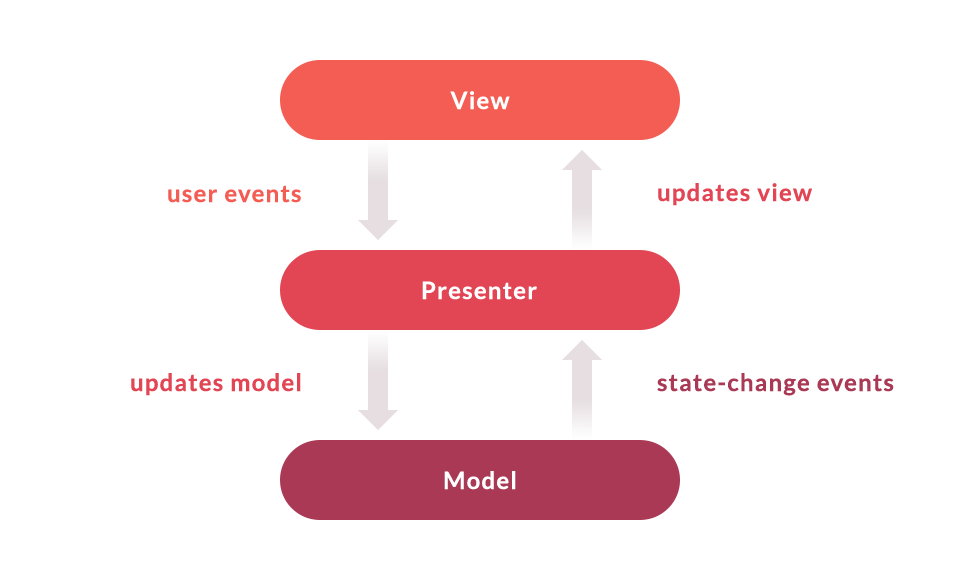
\includegraphics[width=1.0\textwidth]{imagens/model-view-presenter.png}
\legend{Fonte: Macoscope}
\label{fig:model-view-presenter}
\end{figure}

\subsection{API}

O Topin possui duas aplicação independentes em seu modo de desenvolvimento, contudo existe a necessidade de uma interação constante entre as partes, para que possam interagir entre si é necessário o desenvolvimento de uma API, portanto foi determinado o uso da arquitetura REST, como pode ser visto na Figura \ref{fig:rest} este modelo é composto de duas camadas, e para a comunicação entre as camadas foi determinado que os dados seriam transferidos no formato de dados JSON.

\begin{figure}[H]
\caption{Arquitetura REST}
\centering
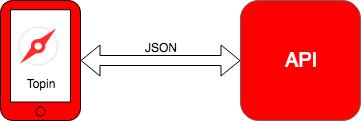
\includegraphics[width=0.6\textwidth]{imagens/rest.png}
\legend{Fonte: Autor}
\label{fig:rest}
\end{figure}

Utilizando a arquitetura REST todos os dados disponíveis na API, serão acessados por meio de endereços eletrônicos com a utilização dos métodos corretos do protocolo HTTP, estes métodos podem ser vistos na Tabela \ref{tab:metodos-http} e, por meio da Tabela \ref{tab:recursos-disponiveis}, é possível visualizar todos os recursos disponibilizados pela API do Topin.

{\renewcommand{\arraystretch}{2}
\begin{table}[H]
\centering
\caption{Recursos Disponíveis na API}
\label{tab:recursos-disponiveis}
\begin{tabular}{ l | p{6cm} | l }
\hline
\textbf{Método} & \textbf{URI} & \textbf{Utilização} \\
\hline
GET & /api/markers & Recupera todos os marcadores. \\ \hline
GET & /api/markers/<id> & Recupera um marcador específico. \\ \hline
GET & /api/lines & Recupera todas as linhas disponíveis \\ \hline
GET & /api/lines/<id> & Recupera uma linha específica \\ \hline
GET & /api/lines/<id>/schedules & Recupera todos os horários de uma linha \\ \hline
POST & /api/complaint & Registra uma nova reclamação \\ \hline
\end{tabular}
\legend{Fonte: Autor}
\end{table}

\section{Tecnologias Utilizadas}

Para a implementação do objeto deste trabalho foram utilizadas várias tecnologias, principalmente pela necessidade de desenvolvimento de três partes distintas que compõem o Topin, o sistema \textit{web}, o aplicativo móvel e a API. A seguir serão demonstradas as tecnologias utilizadas para cada uma destas partes, entretanto como mencionado anteriormente o sistema \textit{web} e a API funcionam de forma conjunta e são implementados em um único \textit{software}, então as tecnologias utilizadas serão apresentadas de forma conjunta.

\subsection*{Sistema Web e API}

{\renewcommand{\arraystretch}{2}
\begin{table}[H]
\centering
\caption{Tecnologias Utilizadas no Sistema Web}
\label{tab:tecnologias-utilizadas-web}
\begin{tabular}{ l | p{11cm} }
\hline
\textbf{Tecnologia} & \textbf{Descrição} \\
\hline
Python\footnotemark & Linguagem de programação orientada a objetos, interpretada e interativa. \\ \hline
Django\footnotemark & O Django é um framework \textit{web} gratuito, de código aberto e de alto nível que incentiva o rápido desenvolvimento e o design limpo e pragmático. \\ \hline
Django Rest Framework\footnotemark & Módulo para o Django que possui um kit de ferramentas poderoso e flexível para criar API's com a arquitetura REST. \\ \hline
GeoDjango\footnotemark & Módulo para o Django que o transforma em um framework \textit{web} geográfico de classe mundial. \\ \hline
PostgreSQL\footnotemark & Poderoso sistema de banco de dados objeto-relacional de código aberto. \\ \hline
PostGIS\footnotemark & Extensão para o PostgreSQL que o transforma em um banco de dados geográfico. \\ \hline
GIT\footnotemark & Sistema de controle de versão distribuído, gratuito e de código aberto projetado para lidar com projetos de pequeno e grande porte. \\ \hline
\end{tabular}
\legend{Fonte: Autor}
\end{table}

\addtocounter{footnote}{-7}
\stepcounter{footnote}\footnotetext{https://www.python.org/}
\stepcounter{footnote}\footnotetext{https://www.djangoproject.com/}
\stepcounter{footnote}\footnotetext{https://www.django-rest-framework.org/}
\stepcounter{footnote}\footnotetext{https://docs.djangoproject.com/en/2.0/ref/contrib/gis/}
\stepcounter{footnote}\footnotetext{https://www.postgresql.org/}
\stepcounter{footnote}\footnotetext{https://postgis.net/}
\stepcounter{footnote}\footnotetext{https://git-scm.com/}

\subsection*{Aplicativo Móvel}

{\renewcommand{\arraystretch}{2}
\begin{table}[H]
\centering
\caption{Tecnologias Utilizadas no Aplicativo Móvel}
\label{tab:tecnologias-utilizadas-movel}
\begin{tabular}{ l | p{11cm} }
\hline
\textbf{Tecnologia} & \textbf{Descrição} \\
\hline
Java\footnotemark & Linguagem de programação para desenvolvimento de aplicações em rede, móveis e incorporadas. \\ \hline
SQLite\footnotemark & Mecanismo de banco de dados SQL autônomo, de alta confiabilidade, incorporado, repleto de recursos e de domínio público. \\ \hline
Room Persistence Library\footnotemark & Biblioteca que fornece uma camada de abstração sobre o SQLite para permitir acesso fluente ao banco de dados, aproveitando todos os recursos do SQLite. \\ \hline
Retrofit2\footnotemark & Biblioteca para abstrair uma API REST em interfaces Java. \\ \hline
Google Maps API\footnotemark & API que possibilita o acesso a todos os recursos do Google Maps. \\ \hline
GIT & Sistema de controle de versão distribuído, gratuito e de código aberto projetado para lidar com projetos de pequeno e grande porte. \\ \hline
\end{tabular}
\legend{Fonte: Autor}
\end{table}

\addtocounter{footnote}{-5}
\stepcounter{footnote}\footnotetext{https://www.java.com/}
\stepcounter{footnote}\footnotetext{https://www.sqlite.org/index.html}
\stepcounter{footnote}\footnotetext{https://developer.android.com/topic/libraries/architecture/room.html}
\stepcounter{footnote}\footnotetext{http://square.github.io/retrofit/}
\stepcounter{footnote}\footnotetext{https://developers.google.com/maps/?hl=pt-br}

\subsection{Python}

Python é uma linguagem de programação de alto nível, no qual suporta vários paradigmas, como orientado a objetos, imperativo, funcional e procedural. É uma linguagem fortemente tipada, como também possui uma tipagem dinâmica. Um dos seus maiores diferenciais se deve ao fato de possuir um código de fácil leitura e exigi a escrita de poucas linhas de código, caso seja comparado a programas, que possuam a mesma finalidade, desenvolvidos em outra linguagem. Como consequência de suas características, o uso desta linguagem se da principalmente no uso de processamento de textos, dados científicos e desenvolvimento de páginas dinâmicas para a \textit{web}.

\subsection{Django}

O Django é um framework de alto nível para a linguagem Python, que incentiva o desenvolvimento rápido, ao mesmo tempo que implementa um projeto de código simples e objetivo. Construído para que os desenvolvedores foquem no que precisa ser desenvolvido sem ter que reinventar a roda, o Django possui uma grande quantidade de mini frameworks embutidos para as mais diversas áreas do desenvolvimento \textit{web}, como por exemplo a criação de API's, a construção de aplicações utilizando dados espaciais entre outros. A seguir são demonstradas algumas características principais que tornaram este framework a ferramenta necessário para o desenvolvimento do Topin.

\begin{figure}[H]
\caption{Arquitetura de Funcionamento do Django}
\centering
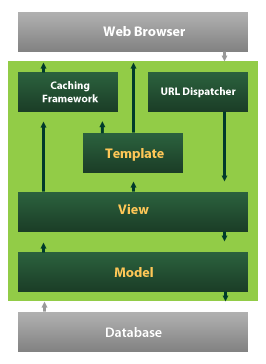
\includegraphics[width=0.6\textwidth]{imagens/django.png}
\legend{Fonte: Chattyhive}
\label{fig:django}
\end{figure}

\subsubsection{Django Rest Framework}

O framework Django REST é um módulo que utilizado juntamente com o Django fornece um kit de ferramentas poderoso e flexível para criar APIs da \textit{web}, pode-se destacar algumas das principais razões para sua utilização no desenvolvimento de API's seguindo a arquitetura REST, são estas:

\begin{lista}
\item A API navegável da \textit{web}, fornecendo um meio gráfico e interativo para verificar o funcionamento da API.
\item Políticas de autenticação, incluindo pacotes para o funcionamento de JWT, OAuth1 e OAuth2.
\item Serialização que suporta fontes de dados ORM e não-ORM.
\item Altamente personalizável, podendo apenas utilizar views baseadas em funções recursos rápidos e simples, a menos que necessário a utilização de recursos mais poderosos.
\item Documentação extensa e excelente suporte da comunidade.
\end{lista}

\subsubsection{GeoDjango}

GeoDjango é um módulo incluído por padrão no Django que o transforma em um framework \textit{web} geográfico de classe mundial. O GeoDjango se esforça para tornar o mais simples possível a criação de aplicativos geográficos da \textit{web}, como serviços baseados em localização. Suas características incluem:

\begin{lista}
\item Tipos de campos para modelos do Django que abordam dados geométricos e geográficos.
\item Extensões ao ORM do Django para consultar e manipular dados espaciais.
\item Interfaces Python de alto nível e pouco acopladas para geometria GIS, bem como possibilita operações de rasterização e manipulação de dados em diferentes formatos.
\end{lista}

\subsection{PostgreSQL}

O PostgreSQL é um sistema de gerenciamento de banco de dados objeto-relacional de código aberto. Possui suporte para todos os principais sistemas operacionais e atende fortemente as características ACID (Atomicidade, Consistência, Integridade e Durabilidade), como também inclui quase todos os tipos de dados: Integer, Numeric, Boolean, Char, Varchar, Date, Interval e Timestamp, bem como o armazenamento de objetos binários grandes e, com isso, suporta o armazenamento de imagens, sons ou vídeos, além de possuir uma boa documentação que fornece suporte a todos os recursos disponíveis.

\subsubsection{PostGIS}

O PostGIS é uma extensão que transforma o PostgreSQL em um banco de dados espacial. Ele adiciona suporte a objetos geográficos, permitindo que consultas de baseadas em localização sejam executadas no SQL. Além do reconhecimento básico de localização, o PostGIS também oferece:

\begin{lista}
\item Funções analíticas e de processamento para dados vetoriais e raster;

\item Álgebra de mapa com dados raster;

\item Funções de reprojeção espacial para dados vetoriais e raster;

\item Suporte para importação e exportação de dados vetoriais;

\item Importação de dados raster;

\item Renderização e importação de funções de suporte a dados vetoriais para formatos textuais;

\item Renderização de dados raster;

\item Funções de chamada SQL de dados raster e vetoriais sem costura para extrusão de valores de pixel por região geométrica, estatísticas de execução por região, recorte de rasters por uma geometria e rasters de vetorização;

\item Suporte a objetos 3D, índice espacial e funções;

\item Suporte a topologia de rede.

\end{lista}
\subsection{Java}

O Java é uma linguagem de programação utilizada para o desenvolvimento de aplicações de todos os tipos, em rede, bem como é amplamente utilizada para a implementação de soluções móveis e embarcadas, como jogos, sistemas para a \textit{internet} e softwares corporativos.

Esta linguagem foi projetada para permitir o desenvolvimento de aplicações multiplataforma de alto desempenho para os mais diversos ambientes de execução. Além de algumas dessas vantagens, o Java se tornou uma importante ferramenta de desenvolvimento, pois permite que os desenvolvedores:

\begin{lista}
\item Armazenem um \textit{software} em uma plataforma e o executem virtualmente em qualquer outro ambiente.
\item Implementem softwares para a \textit{internet}.
\item Integre aplicações e serviços utilizando a linguagem para desenvolver aplicações personalizáveis.
\item Desenvolva sistemas de alto desempenho e eficientes para celulares, processadores remotos, microcontroladores, módulos sem fio, sensores, \textit{gateways}, produtos de consumo geral entre outros dispositivos.
\end{lista}

\subsection{SQLite}

SQLite é uma biblioteca de código aberto e domínio público que implementa um banco de dados SQL transacional incorporado. Ao contrário da maioria dos outros bancos de dados SQL, o SQLite não possui um processo de servidor separado. O SQLite lê e grava diretamente em arquivos de disco comuns. Um banco de dados SQL completo com várias tabelas, índices, acionadores e visualizações está contido em um único arquivo de disco. O formato de arquivo de banco de dados é multi-plataforma. Esses recursos tornam o SQLite uma escolha popular como um formato de arquivo de aplicativo.

O SQLite é uma biblioteca compacta. Com todos os recursos ativados, o tamanho da biblioteca pode ser menor que 500 KB, dependendo da plataforma de destino e das configurações de otimização do compilador. Há uma compensação entre o uso de memória e a velocidade. O SQLite geralmente roda mais rápido quanto mais memória você der. No entanto, o desempenho geralmente é bom mesmo em ambientes com pouca memória. Dependendo de como é usado, o SQLite pode ser mais rápido que a E/S do sistema de arquivos direto.

O SQLite é testado com muito cuidado antes de cada lançamento e tem a reputação de ser muito confiável. A maior parte do código fonte do SQLite é dedicada apenas a testes e verificações. Um conjunto de testes automatizado executa milhões e milhões de casos de teste envolvendo centenas de milhões de instruções SQL individuais e atinge 100\% de cobertura de teste de filial. O SQLite responde normalmente às falhas de alocação de memória e erros de E/S de disco. As transações são ACID mesmo que seja interrompido por falhas no sistema ou falhas de energia.

\subsection{GIT}

O Git é um sistema de controle de versão distribuído gratuito e de código aberto projetado para lidar desde projetos pequenos a projetos grandes e complexos, com velocidade e eficiência. As principais características do GIT são:

\begin{lista}
\item \textbf{Ramificação e fusão:} Este recurso permite que o desenvolvedor tenha várias ramificações locais que podem ser totalmente independentes umas das outras.
\item \textbf{Pequeno e Rápido:} Quase todas as operações são realizadas localmente, proporcionando uma enorme vantagem de velocidade em relação a sistemas centralizados que constantemente precisam se comunicar com um servidor.
\item \textbf{Distribuído:} Consiste em um sistema de controle de versão que, em vez de manter apenas a versão atualizada do código, ele copia na integra todo o repositório do servidor, incluindo as versões atuais e anteriores do sistema.
\item \textbf{Integridade dos dados} O modelo de dados que o Git usa garante a integridade criptográfica de cada bit do seu projeto.
\item \textbf{Área de preparação:} Área intermediária onde suas modificações podem ser formatadas e revisadas localmente antes de serem enviados ao repositório compartilhado.
\end{lista}

\begin{figure}[H]
\caption{Arquitetura de Funcionamento do GIT}
\centering
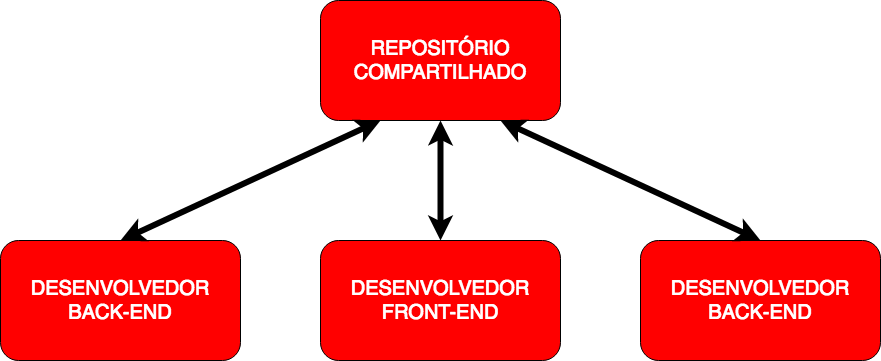
\includegraphics[width=0.8\textwidth]{imagens/git.png}
\legend{Fonte: Autor}
\label{fig:git}
\end{figure}

\section{Funcionalidades}

Nesta sessão são apresentadas as principais funcionalidades do Topin. Para a efetivação desse trabalho foi desenvolvido dois módulos: sistema de gerenciamento da empresa de transporte público e o aplicativo móvel para os passageiros.

Para o entendimento das funcionalidades se faz necessária a compreensão de alguns aspectos do funcionamento do transporte público, como: linhas, trajetos, horários, marcadores e reclamações.

\begin{lista}
\item \textbf{Linhas:} São as rotas disponibilizadas pela empresa de transporte coletivo, onde deve ser especificada a parada inicial e a parada final de cada linha.
\item \textbf{Trajeto:} São as coordenadas geográficas de todos os pontos de referência, geralmente são coletadas principalmente as coordenadas geográficas de cada curva do caminho percorrido.
\item \textbf{Horários:} São todos os horários de saída do veículo da origem das linhas disponíveis, com base na hora de partida e o dia da semana que este horário está disponível.
\item \textbf{Marcadores:} São todos os pontos de interesse do usuário, basicamente é composto por paradas, em que é possível pegar o transporte, e pontos de venda de bilhetes, onde é possível efetuar a compra de bilhetes para o uso do transporte público.
\item \textbf{Reclamações:} É a mensagem deixada por um passageiro que tenha passado por algum inconveniente ou apenas deseja deixar seu comentário sobre sua experiência com o transporte público.
\end{lista}

\subsection{Administradores de Empresa de Transporte Público}

Os administradores da empresa de transporte público possuem um papel vital para o funcionamento do Topin, pois possuem a responsabilidade de registrar e gerir as informações que serão disponibilizadas aos passageiros, como pode ser visto na Figura \ref{fig:empresa-cadastro-linha} os administradores devem cadastrar todos os detalhes referentes as linhas dos transportes, bem como devem registrar os marcadores desta mesma linha, para que assim os passageiros visualizem apenas os marcadores que serão uteis no uso desta linha.

\begin{figure}[t]
\caption{Topin para Empresa - Tela de Cadastro da Linha}
\centering
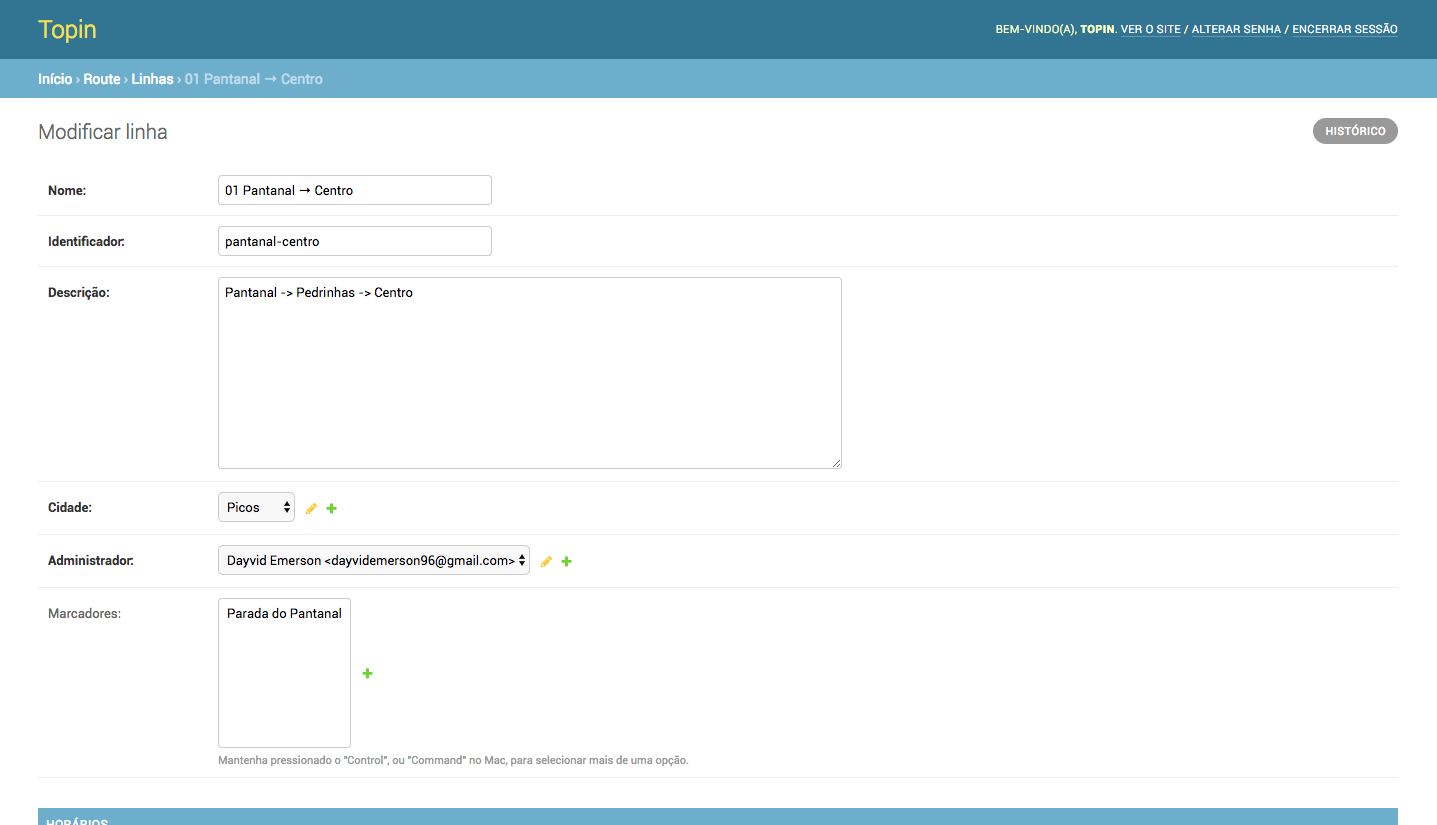
\includegraphics[width=1.0\textwidth]{imagens/cadastro-linha.png}
\legend{Fonte: Autor}
\label{fig:empresa-cadastro-linha}
\end{figure}

Ainda no cadastro das linhas é possível visualizar na Figura \ref{fig:empresa-cadastro-horarios-trajeto} que os administradores também deverão informar os horários disponíveis para o transporte público e, não apenas registrar os horários, como também separar estes horários por dia da semana, para que não exista a possibilidade do usuário ser informado de um horário que não estará disponível no fim de semana, por exemplo.

Ao registrar os horários, a forma de registro dos dias da semana se destaca, pois para esta aplicação foi criado um campo no banco de dados PostgreSQL do tipo lista de valores, que se trata de um tipo de campo onde é permitido salvar um conjunto de valores sem que exista a necessidade criação de uma nova tabela para tal objetivo, por esse motivo o registro dos dias da semana para ser compatível com o banco de dados é colocado em uma cadeia de caracteres com os valores separados por vírgula, as opções de dias da semana são: \textit{sunday, monday, tuesday, wednesday, thursday, friday, saturday}.

Ao visualizar a Figura \ref{fig:empresa-cadastro-horarios-trajeto} pode-se observar que além dos horários, o administrador irá registrar todos os pontos de uma linha, contudo estes pontos são referentes ao trajeto, ou seja, o caminho percorrido pelo transporte na linha em questão. Geralmente, os pontos de referência escolhidos são baseados em sua localização no mapa para formar o desenho do trajeto possível, como por exemplo são colocadas as coordenadas geográficas apenas das curvas do trajeto, para os perfeccionistas é possível registrar todas as coordenadas do trajeto, o que pode facilmente passar de 200 coordenadas geográficas.

\begin{figure}[H]
\caption{Topin para Empresa - Tela de Cadastro dos Horários e Trajeto da Linha}
\centering
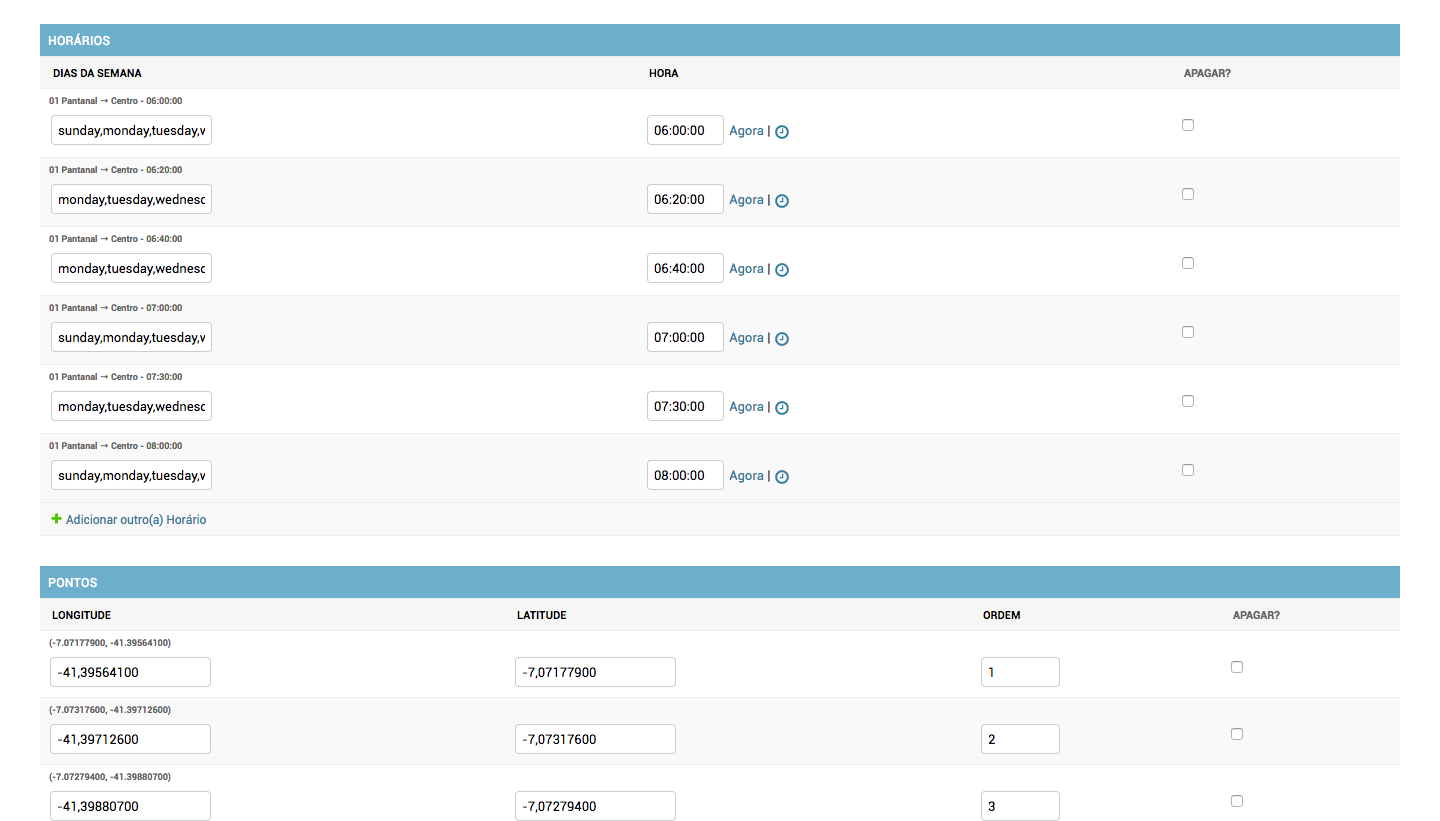
\includegraphics[width=1.0\textwidth]{imagens/cadastro-horarios-pontos.png}
\legend{Fonte: Autor}
\label{fig:empresa-cadastro-horarios-trajeto}
\end{figure}

Os marcadores são pontos de interesse no uso de transporte público e para os administradores é disponibilizado um meio de registro desses pontos, ao analisar a Figura \ref{fig:empresa-cadastro-ponto} é perceptível a possibilidade do administrador da empresa registrar a localização do marcador, bem como é possível informar uma descrição do marcador no intuito de informar ao passageiros mais detalhes sobre o ponto registrado.

\begin{figure}[H]
\caption{Topin para Empresa - Tela de Cadastro dos Marcadores}
\centering
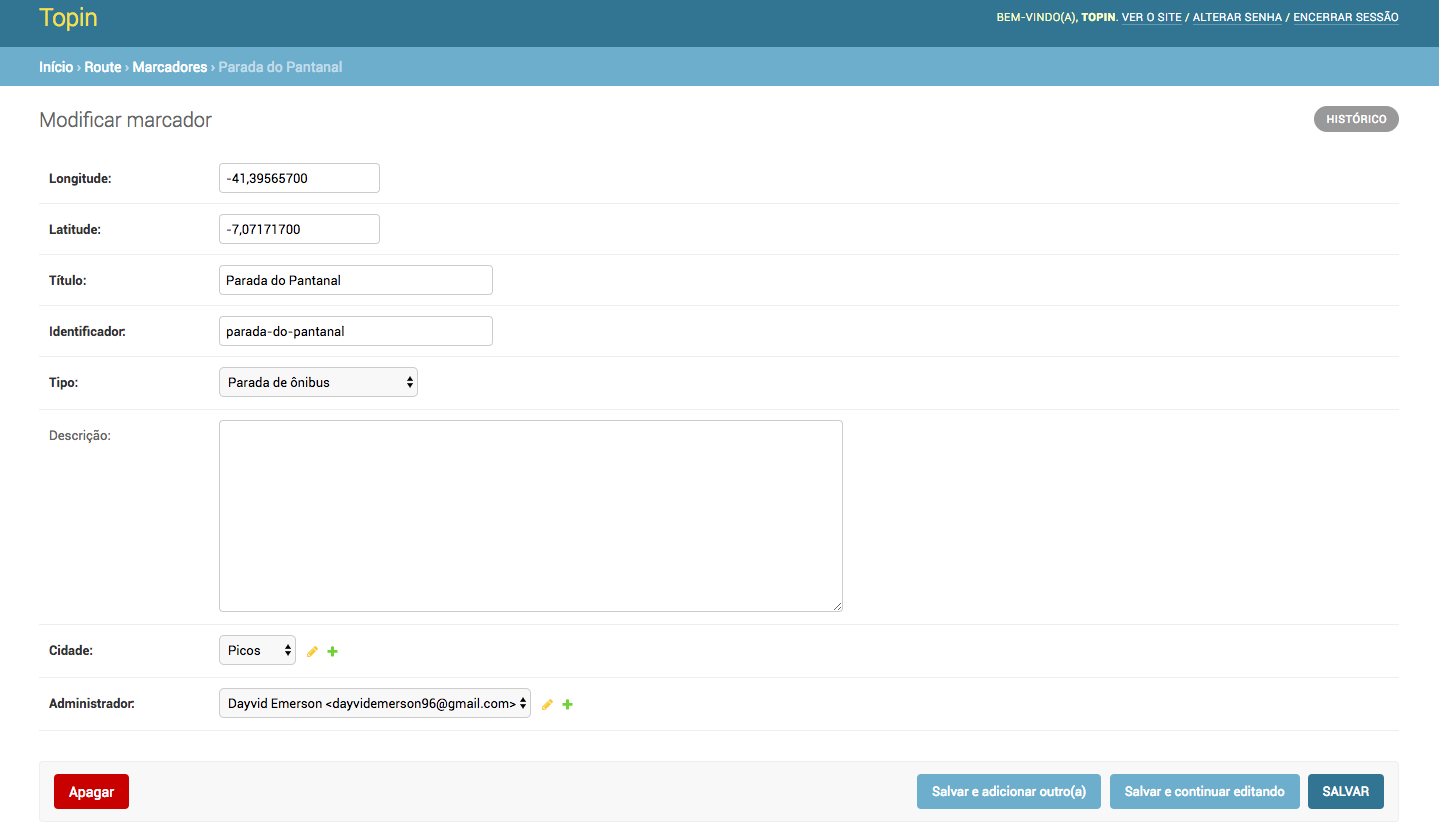
\includegraphics[width=1.0\textwidth]{imagens/cadastro-ponto.png}
\legend{Fonte: Autor}
\label{fig:empresa-cadastro-ponto}
\end{figure}

Um dos principais problemas descritos nesse trabalho se deve a dificuldade dos passageiros entrarem em contato com as pessoas
responsáveis pelo transporte público para descrever a sua indignação com o serviço prestado de alguma forma, como já foi
demonstrado neste projeto os passageiros, muitas vezes, não sabem a quem reclamar e acabam culpando pessoas ou instituições
que não tem autoridade para solucionar o problema encontrado.

Como pode ser visto na Figura \ref{fig:empresa-visualizar-reclamacao}, visando este problema foi disponibilizada aos
administradores das empresas de transporte público uma seção onde eles podem acompanhar as reclamações que os passageiros
enviaram por meio do aplicativo Topin.

\begin{figure}[H]
\caption{Topin para Empresa - Tela de Visualização das Reclamações}
\centering
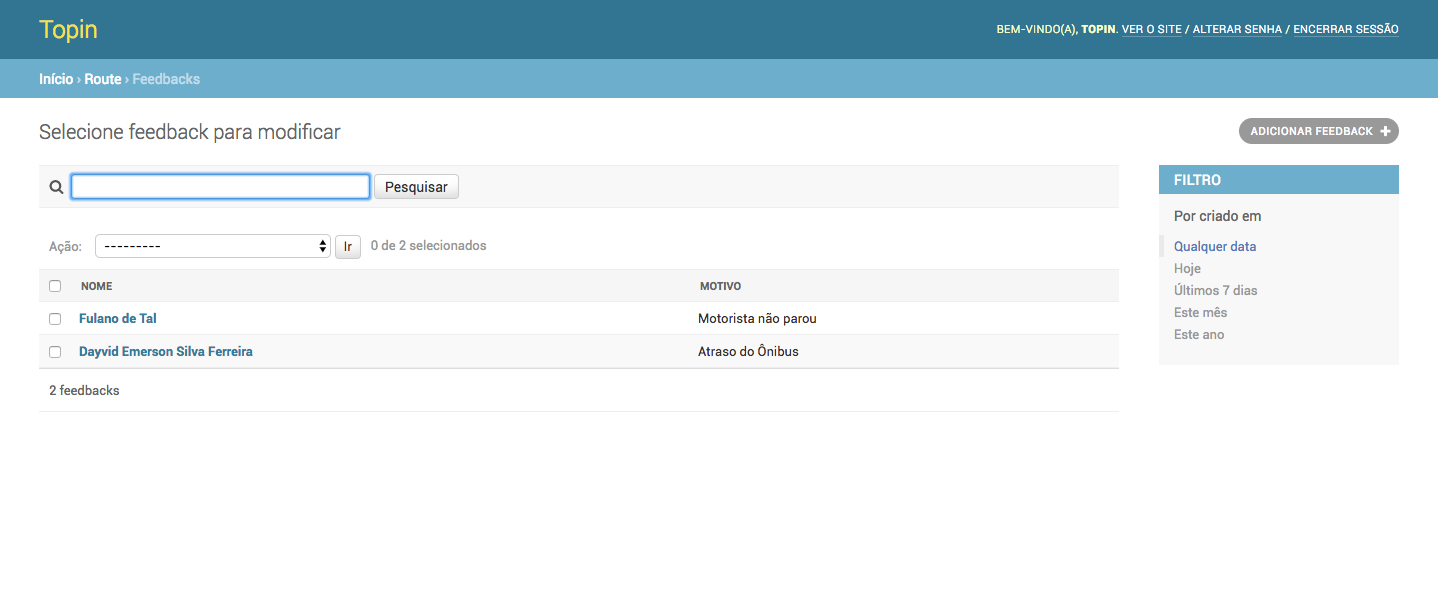
\includegraphics[width=1.0\textwidth]{imagens/visualizar-reclamacao.png}
\legend{Fonte: Autor}
\label{fig:empresa-visualizar-reclamacao}
\end{figure}

\subsection{Passageiro}

O aplicativo criado para o uso dos passageiros de transporte coletivo possui o objetivo de informá-los sobre detalhes referentes
ao funcionamento do serviço de transporte público, porém antes de explicar as funcionalidades do aplicativo vale ressaltar
que o aplicativo permite a visualização das informações sem a necessidade do uso de \textit{internet}, por ser um recurso que funciona em
segundo plano não existe a possibilidade de demonstrá-lo graficamente.

Entretanto todos os dados mostrados no aplicativo são consultados na API do Topin, em que necessita do uso de uma rede de dados,
contudo o aplicativo ao recebê-los automaticamente os salva no banco de dados do \textit{smartphone}, permitindo verificar em um
acesso posterior se há \textit{internet} disponível no dispositivo ou se foi encontrado algum erro na consulta das informações, caso isso
aconteça, serão exibidos os dados armazenados no \textit{smartphone} e, com isso, garantir que os passageiros terão acesso as
informações que precisa mesmo que não possua \textit{internet} disponível no momento.

Uma das funcionalidades principais do aplicativo pode ser vista na Figura \ref{fig:passageiro-linhas-disponiveis} onde é possível
perceber a presença de um espaço que permite visualizar todas as linhas disponíveis para uso do transporte público na região,
além de dividir essas informações com um mapa demonstrando sua localização atual.

Também é permitido ao usuário arrastar a lista das linhas para cima possibilitando a visualização apenas das linhas disponíveis
ocupando todo o espaço disponível na tela do \textit{smartphone} ou como demonstrado na Figura \ref{fig:passageiro-visualizacao-linha}
é possível deslizar a lista de linhas para baixo fazendo com que o mapa preencha toda a tela do aparelho, portanto o passageiro poderá
ter uma visualização ampla da sua posição atual em relação as paradas e o trajeto da linha selecionada.

\begin{figure}[H]
\caption{Topin para Passageiros - Tela de Visualização das Linhas Disponíveis}
\centering
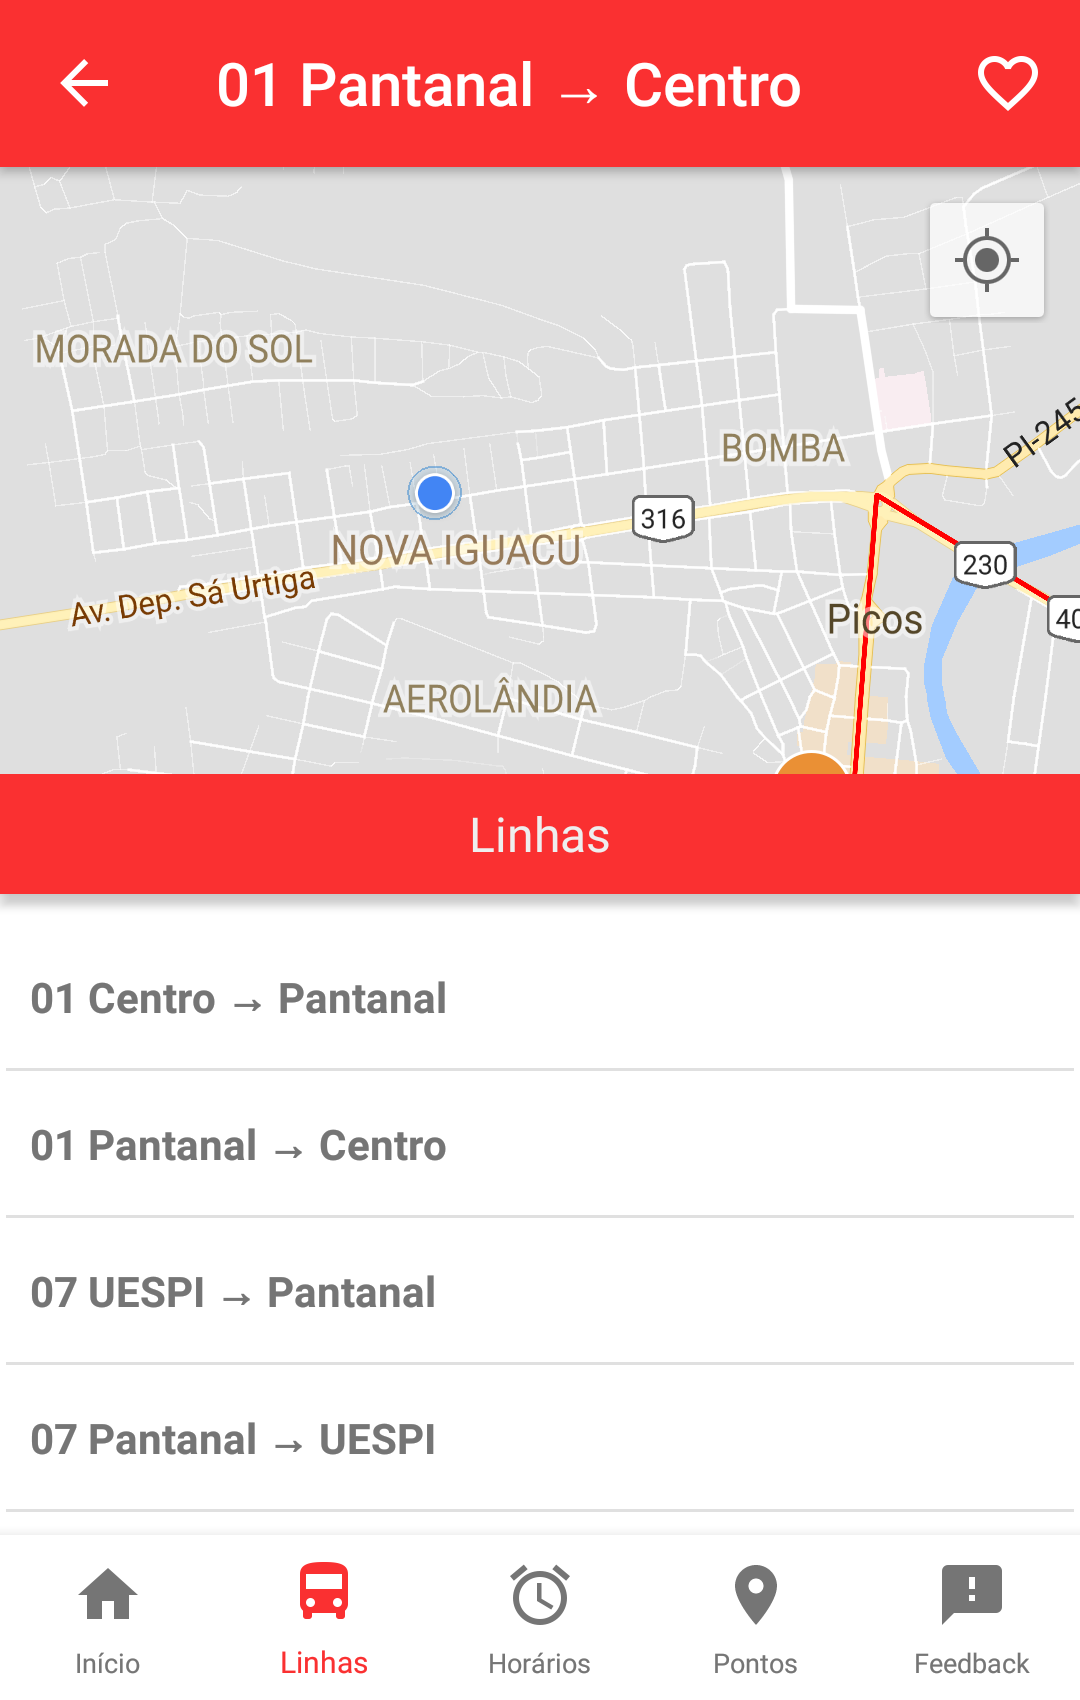
\includegraphics[width=0.3\textwidth]{imagens/linhas-disponiveis.png}
\legend{Fonte: Autor}
\label{fig:passageiro-linhas-disponiveis}
\end{figure}

\begin{figure}[H]
\caption{Topin para Passageiros - Tela de Visualização da Linha Selecionada}
\centering
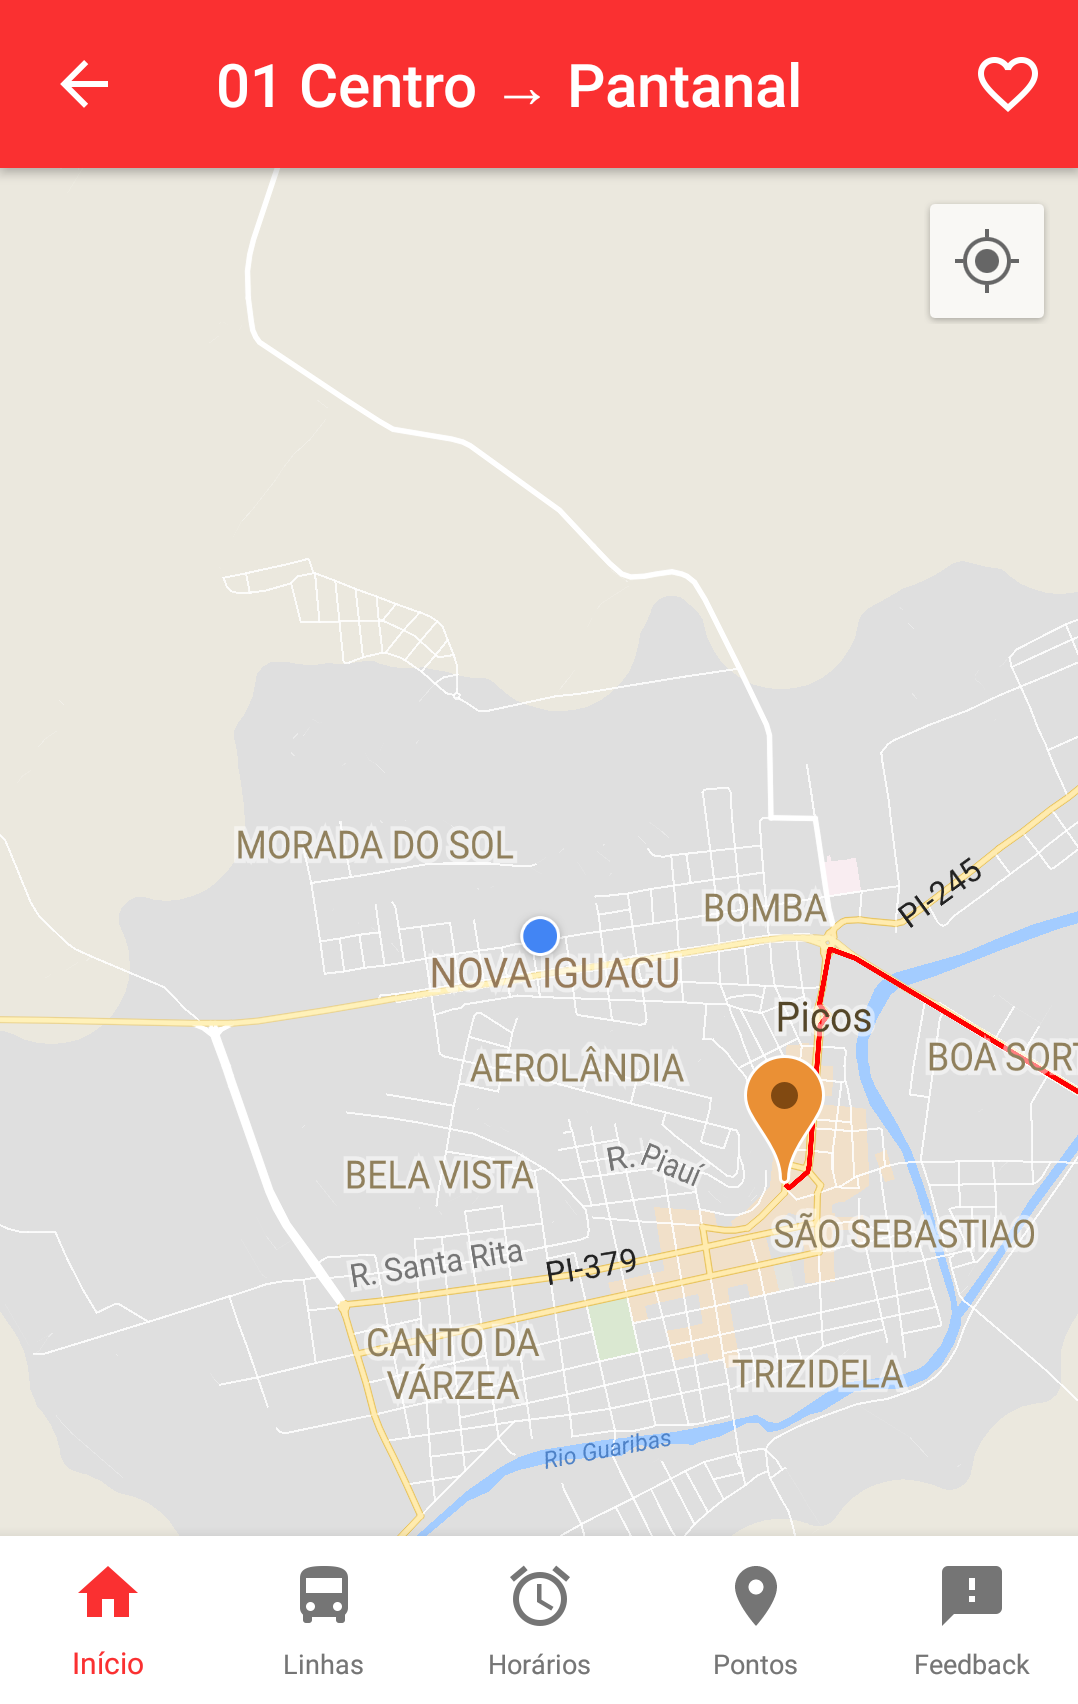
\includegraphics[width=0.3\textwidth]{imagens/visualizacao-linha.png}
\legend{Fonte: Autor}
\label{fig:passageiro-visualizacao-linha}
\end{figure}

Ao observar a Figura \ref{fig:passageiro-horarios-linha} é perceptível a presença do mesmo recurso existente
para a lista de linhas, recurso este que possibilita a lista de horários ser arrastada tanto para cima, como
para baixo, para destacar a visualização de um dos componentes da tela que está dividida.

O passageiro ao consultar a lista de horários automaticamente é demonstrado os horários do dia da semana baseado
na data atual do \textit{smartphone}, no entanto é permitido ao usuário alternar entre os dias da semana, que ao
selecionar um dia da semana diferente será mostrado apenas o ponto de partida e os horários disponíveis para aquele
dia da semana específico, como por exemplo a terça-feira que está selecionada na Figura \ref{fig:passageiro-horarios-linha}
é possível visualizar todos os horários disponíveis e a origem a partir do ponto de partida da linha, nesse
caso específico, a parada do Centro.

\begin{figure}[H]
\caption{Topin para Passageiros - Tela de Visualização dos Horários da Linha}
\centering
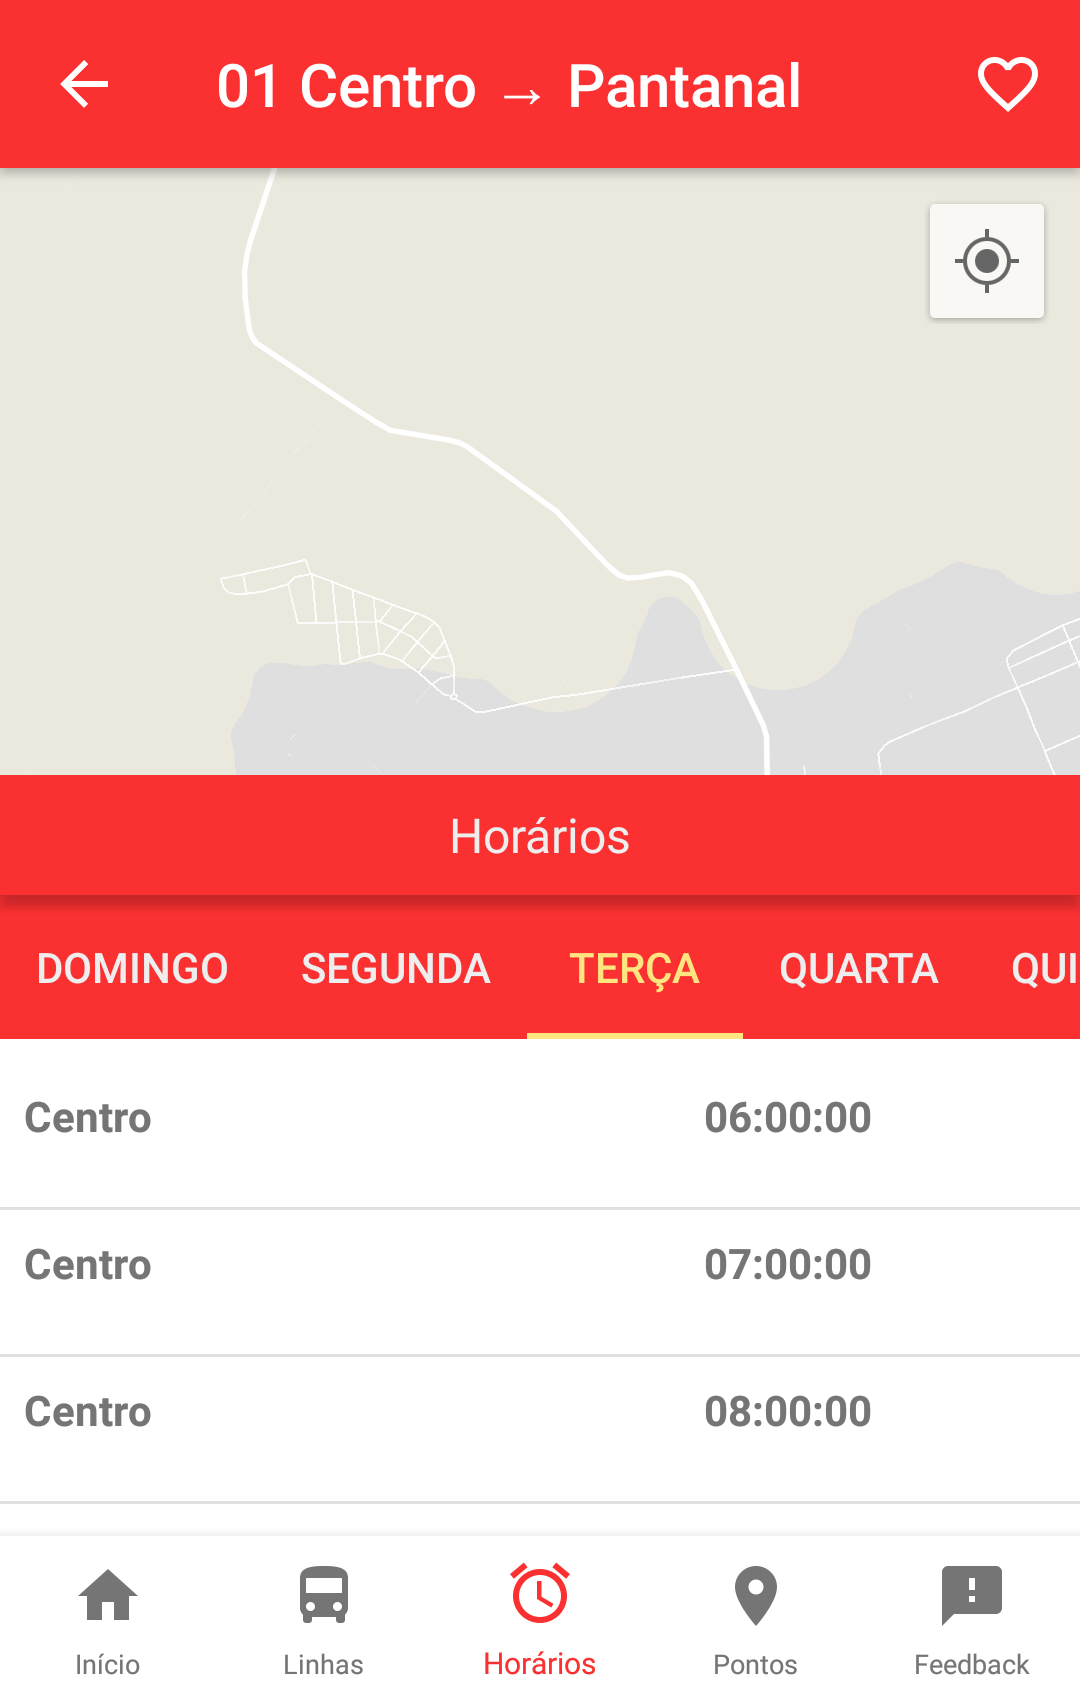
\includegraphics[width=0.3\textwidth]{imagens/horarios-linha.png}
\legend{Fonte: Autor}
\label{fig:passageiro-horarios-linha}
\end{figure}

Pode-se visualizar na Figura \ref{fig:passageiro-pontos-linha} que é possível visualizar os marcadores de interesse para a linha selecionada, em que é demonstrado no mapa por meio de um ícone todos os marcadores listados, ou seja, é visível não apenas a lista dos pontos de interesses, como também a sua geolocalização no mapa, e por meio do uso de sua localização atual, os passageiros podem se deslocar com uma maior facilidade para o ponto desejado.

Como dito anteriormente nesse trabalho uma das dificuldades encontradas pelos passageiros é a entrega de reclamações
para as pessoas responsáveis pela prestação do serviço. Para alcançar esse objetivo é disponibilizado aos usuários
do aplicativo móvel um ambiente (Figura \ref{fig:passageiro-feedback}) em que é possível enviar uma mensagem que
será entregue as autoridades que competem a responsabilidade pela boa ou má prestação do serviço de transporte público.

\begin{figure}[H]
\caption{Topin para Passageiros - Tela de Visualização dos Pontos da Linha}
\centering
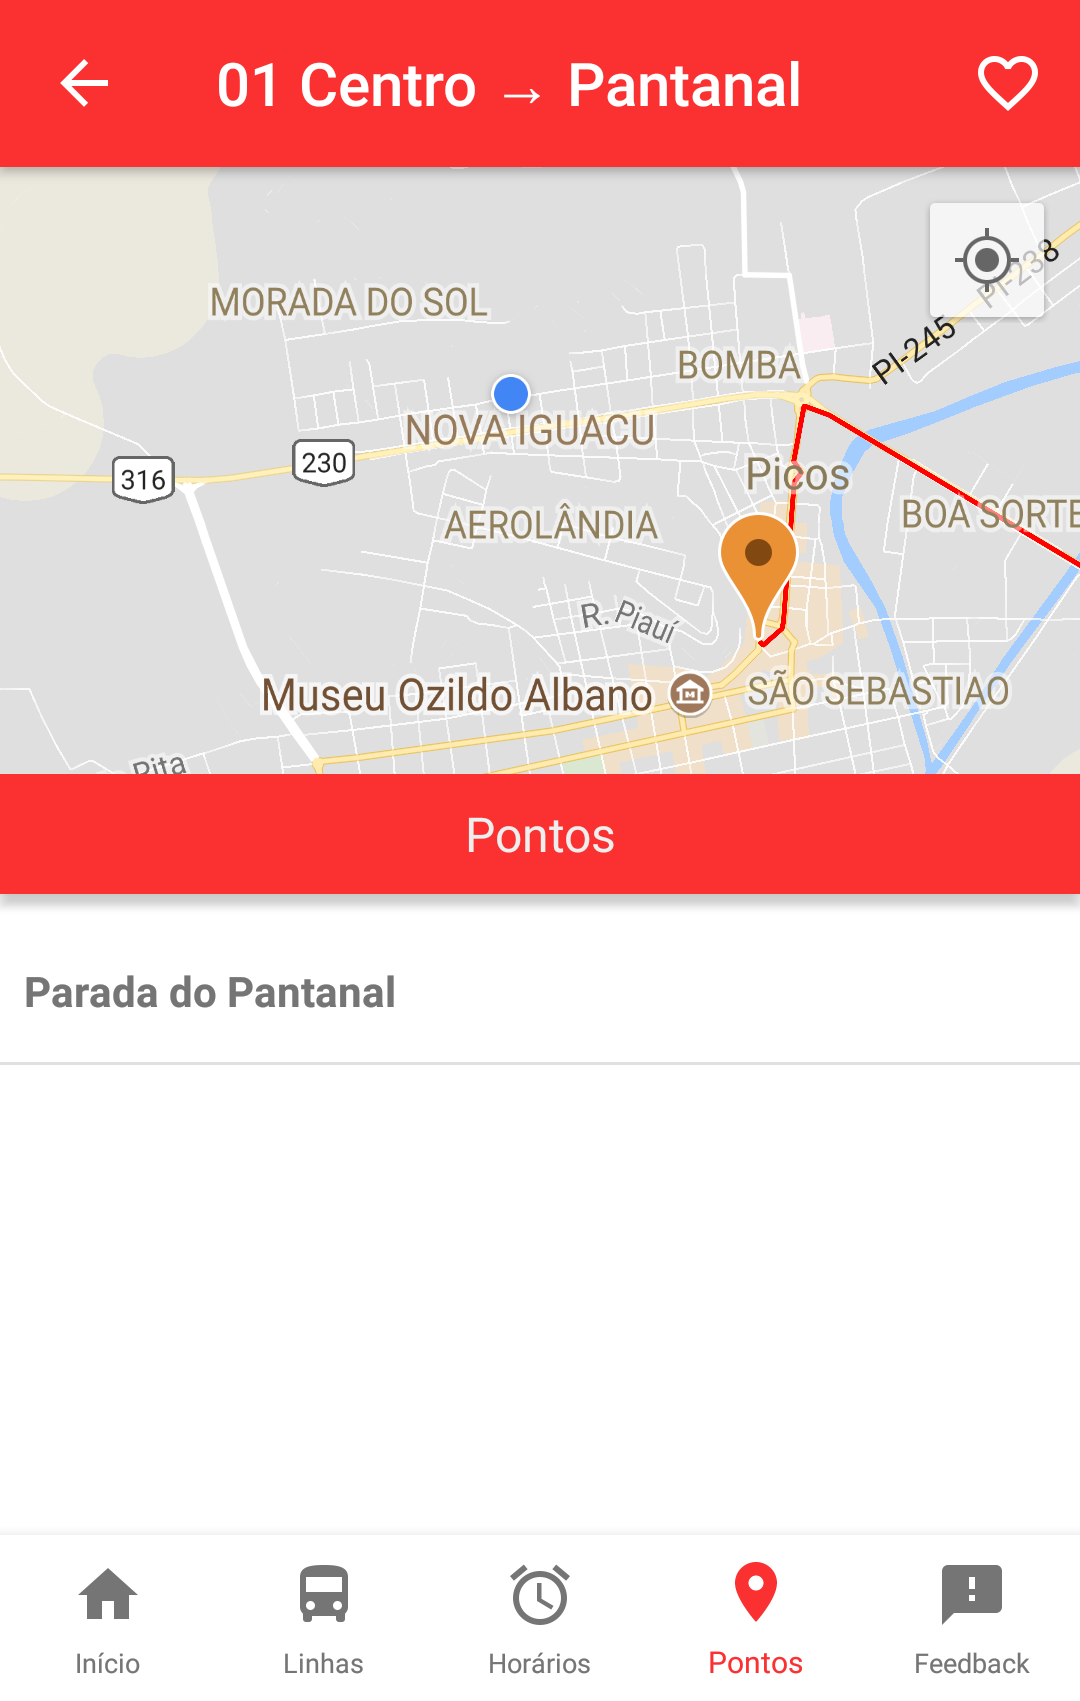
\includegraphics[width=0.3\textwidth]{imagens/pontos-linha.png}
\legend{Fonte: Autor}
\label{fig:passageiro-pontos-linha}
\end{figure}

\begin{figure}[H]
\caption{Topin para Passageiros - Tela de Registro de Feedback}
\centering
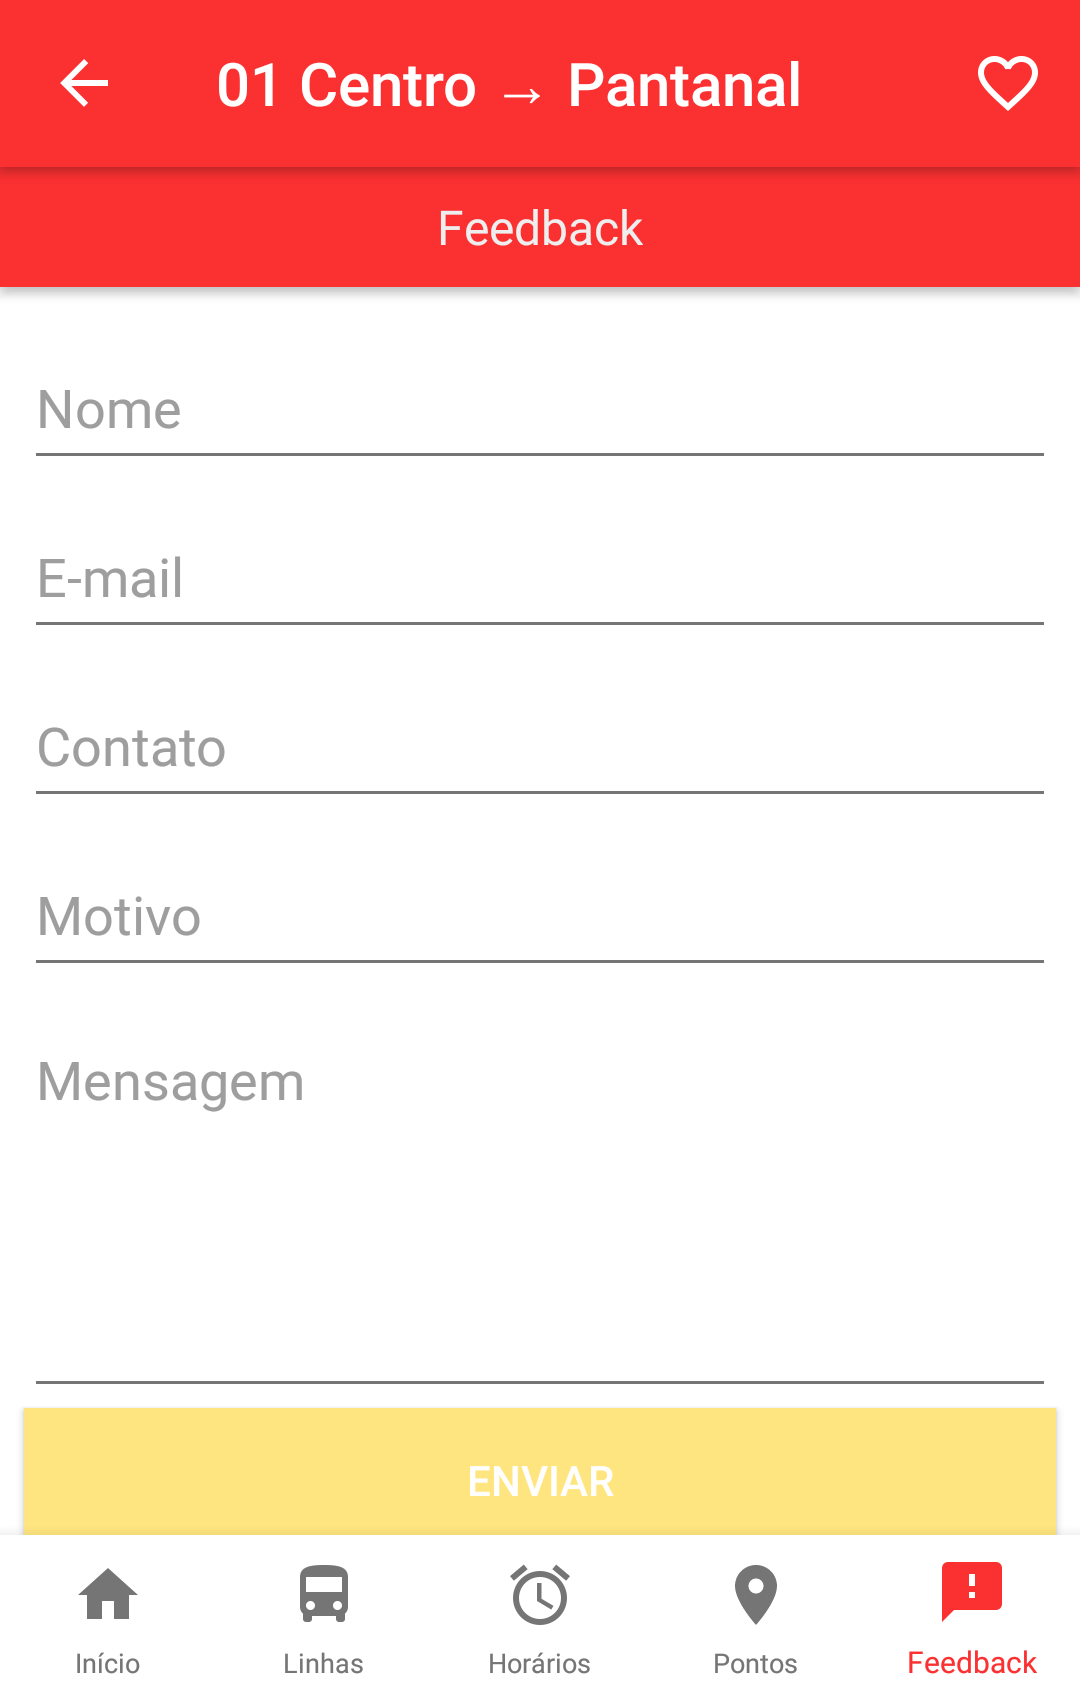
\includegraphics[width=0.3\textwidth]{imagens/feedback.png}
\legend{Fonte: Autor}
\label{fig:passageiro-feedback}
\end{figure}